\begin{defi}
    Soit $A = (a_{i,j}) \in \M_n(\K)$. On dit que $A$ est 
    \begin{itemize}
        \item à \emph{diagonale dominante} si
        $$\forall i \in \llbracket 1, n \rrbracket,\ |a_{i,i}| \geqslant \sum_{k \not = i} |a_{i,k}|,$$
        \item à \emph{diagonale fortement dominante} si de plus l'inégalité est stricte pour une valeur de $i$ au moins,
        \item à \emph{diagonale strictement dominante} si l'inégalité est stricte pour tout $i$. 
    \end{itemize}
\end{defi}

\begin{lemme} \label{lemme_hadamard}
    Toute matrice à diagonale strictement dominante (DSD) est inversible.
\end{lemme}

\marginnote[2cm]{
    \begin{methode}
    Penser à poser 
        $$\left |x_{i_0} \right | \defeq \max_{1 \leqslant i \leqslant n} |x_i|.$$
    \end{methode}
}

\begin{preuve}
    Soit $X = \Trsp{(x_1 \cdots x_n)} \in \Ker(A)$. \\
    On pose $\displaystyle \left |x_{i_0} \right| \defeq \max_{1 \leqslant i \leqslant n} |x_i|$. La ligne $i_0$ de la relation $AX = 0$ donne
    $$\sum_{j=1}^n a_{i_0,j}x_j = 0$$
    soit
    $$-a_{i_0, i_0} x_{i_0} = \sum_{j \not = i_0} a_{i_0,j} x_j$$
    d'où, d'après l'inégalité triangulaire,
    $$|a_{i_0, i_0}| |x_{i_0}| \leqslant \sum_{j \not = i_0} |a_{i_0,j}| |x_j| \leqslant |x_{i_0}| \sum_{j \not = i_0} |a_{i_0, j}|.$$
    Comme $|a_{i_0, i_0}| > \sum\limits_{j \not = i_0} |a_{i_0, j}|$ par définition de $A$, on en déduit que
    $|x_{i_0}| = 0$, autrement dit $X = 0$. Le noyau de $A$ est donc réduit au vecteur i.e. la matrice $A$ est inversible. \\
    Pour une autre démonstration voir \cite{matrices} page 51. 
\end{preuve}

\marginnote{
    On considère la matrice à coefficients complexes
    $$
    \begin{pmatrix}
        \textcolor{red}{\mi4} & 0 & 2 & \mi3 \\
        1 & \textcolor{blue}{5+\mi10} & 5 & -1 \\
        0 & 2 & \textcolor{ForestGreen}{1} & 0 \\
        1 & 2 & 0 & \textcolor{orange}{-8-\mi2}
    \end{pmatrix}.
    $$
    Ci-dessous sont représentés ses disques de \textsc{Gerschgorin} et les croix correspondent à ses valeurs propres.
}

\begin{marginfigure}
    % This file was created with tikzplotlib v0.10.1.
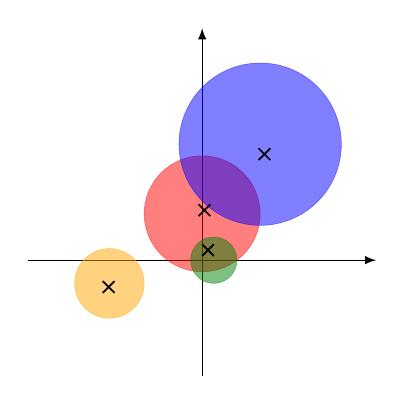
\begin{tikzpicture}

\definecolor{dimgray85}{RGB}{85,85,85}
\definecolor{gainsboro229}{RGB}{229,229,229}
\definecolor{green}{RGB}{0,128,0}
\definecolor{lightgray204}{RGB}{204,204,204}
\definecolor{orange}{RGB}{255,165,0}

\begin{axis}[
axis lines=middle,
inner axis line style={-latex},
grid=major,
width=6cm,
height=6cm,
xtick=\empty,
xmin=-15, xmax=15,
ytick=\empty,
ymin=-10, ymax=20,
]
\draw[draw=red,fill=red,opacity=0.5,very thin] (axis cs:0,4) circle (5);
\draw[draw=blue,fill=blue,opacity=0.5,very thin] (axis cs:5,10) circle (7);
\draw[draw=green,fill=green,opacity=0.5,very thin] (axis cs:1,0) circle (2);
\draw[draw=orange,fill=orange,opacity=0.5,very thin] (axis cs:-8,-2) circle (3);

\def\r{3}

%\addplot [semithick, red, mark=*, mark size=\r, mark options={solid}, only marks]
%table {%
%0 4
%};
%\addlegendentry{1\mi}
%\addplot [semithick, blue, mark=*, mark size=\r, mark options={solid}, only marks]
%table {%
%5 10
%};
%\addlegendentry{(5+10\mi)}
%\addplot [semithick, green, mark=*, mark size=\r, mark options={solid}, only marks]
%table {%
%1 0
%};
%\addlegendentry{(1)}
%\addplot [semithick, orange, mark=*, mark size=\r, mark options={solid}, only marks]
%table {%
%-8 -2
%};
%\addlegendentry{(-8-2j)}

\addplot [semithick, black, mark=x, mark size=\r, mark options={solid}, only marks, forget plot]
table {%
-8.06720901070025 -2.31297809243462
};
\addplot [semithick, black, mark=x, mark size=\r, mark options={solid}, only marks, forget plot]
table {%
5.36805383956579 9.13980083948909
};
\addplot [semithick, black, mark=x, mark size=\r, mark options={solid}, only marks, forget plot]
table {%
0.195375871819944 4.3072164295875
};
\addplot [semithick, black, mark=x, mark size=\r, mark options={solid}, only marks, forget plot]
table {%
0.503779299314509 0.865960823358021
};
\end{axis}

\end{tikzpicture}
\end{marginfigure}

\begin{theo}
    Soit $A \in \M_n(\K)$. Alors, $$\Sp(A) \subset \bigcup\limits_{i=1}^{n} \overline{\mathscr{B}} \Bigg( a_{i,i}, \sum\limits_{k \not = i} |a_{i,k}| \Bigg).$$ \\
    Ces disques sont nommés les \href{https://fr.wikipedia.org/wiki/Théorème_de_Gerschgorin}{disques de \textsc{Gerschgorin}} (cf. thème \textit{Localisation des valeurs propres}, Ch. 11 \cite{acamanes}).
\end{theo}

\begin{preuve}
    Soit $\lambda \in \Sp(A)$. La matrice $A - \lambda \I_n$ n'est pas inversible donc n'est pas à DSD i.e. pour tout $i \in \llbracket 1, n \rrbracket$,
    $$|a_{i,i} - \lambda| \leqslant \sum_{k \not= i} |a_{i,k}|.$$
    Le spectre de la matrice $A$ est donc inclus dans la réunion des disques de centre $a_{i,i}$ et de rayon $\sum\limits_{k \not=i} a_{i,k}$.
\end{preuve}    

\begin{corol}
    Soit $A \defeq (a_{i,j})_{1 \leqslant i, j \leqslant n} \in \M_n(\K)$. On note
    \begin{equation*}
        E &\defeq \bigcup\limits_{i=1}^{n} \overline{\mathscr{B}} \Bigg( a_{i,i}, \sum\limits_{k \not = i} |a_{i,k}| \Bigg) \quad
        E' &\defeq \bigcup\limits_{i=1}^{n} \overline{\mathscr{B}} \Bigg( a_{i,i}, \sum\limits_{j \not = i} |a_{j, i}| \Bigg).
    \end{equation*}
    Alors,
    $$\Sp(A) \subset E \cap E'.$$
\end{corol}

\begin{preuve}
    D'après le théorème 4.1 (lien), 
    $$\Sp(A) \subset E \text{ et } \Sp(\Trsp{A}) \subset E'.$$
    Or $\Sp(A) = \Sp(\Trsp{A})$ donc $\Sp(A) \subset E \cap E'$.
\end{preuve}

\begin{prop}
    Soit $A \in \M_n(\R)$ à DSD telle que $a_{i,i} > 0$ pour tout $i \in \llbracket 1, n \rrbracket$. Alors $\mathrm{det}(A) > 0$. 
\end{prop}

\begin{preuve}
        $\det(A) = \prod\limits_{\lambda \in \Sp(A)} \lambda$. Distinguer les vap complexes et réelles...
\end{preuve}
